% RESUMEN

\chapter{Overview}
%\addcontentsline{toc}{chapter}{Overview}
%\markboth{Overview}{Overview}


Petri nets (PNs)\cite{ARMura89,BODHPSV93} is a mathematical formalism for the description of discrete-event systems, that has been successfully used for modeling, analysis and synthesis purposes of such systems. A key feature of a
PN is that its structure can capture graphically fundamental primitives in concurrency theory such as parallelism,
synchronization, mutual exclusion, etc. The state of a PN system is given by a vector of non-negative
integers representing the marking of its places.

As any other formalism for discrete event systems, PNs suffer from the \emph{state explosion problem} which produces an exponential growth of the size of the state space with respect to the initial marking. One way to avoid the state explosion is to relax the integrality constraint in the firing of transitions and deal with transitions that are fired in real amounts. A transition whose firing amount is allowed to be any real number between zero and its enabling degree is said to be a \emph{continuous transitions}. The firing of a continuous transition can produce a real, not integer, number of tokens in its input and output places. If all transitions of a net are continuous, then the net is said to be continuous. If a non-empty proper subset of transitions is continuous, then the net is said to be hybrid \cite{BODavid10}.

Different time interpretations can be considered for the firing of continuous transitions. The most popular ones are infinite and finite server semantics which represent a first order approximation of the firing frequency of discrete transitions. For a broad class of Petri nets, infinite server semantics offers a better approximation of the steady-state throughput  than finite server semantics \cite{ARMARESI09}. Moreover, finite server semantics can be exactly mimicked by infinite server semantics in discrete transitions simply by adding a self-loop place. A third firing semantics, called product semantics, is also frequently used when dealing with biochemical and population dynamics systems.

$SimHPN$ is a MATLAB embedded software that provides support for infinite server and product semantics in both, discrete and continuous, types of transition. A description of a preliminary version of this software can be found in~\cite{JuMa10,JuMaVa11,simhpn2012806}. This is the first MATLAB package that enables the analysis and simulation of hybrid nets with these two firing semantics. There already exists a toolbox dealing with discrete Petri nets~\cite{IPMaMaPa03c}, and one for the so-called first order hybrid Petri nets~\cite{ICSeGiSe08} which provides support for continuous transitions under finite server semantics. The main features of the $SimHPN$ toolbox are: 
\begin{enumerate}
\item simulation of hybrid Petri nets under different server semantics; 
\item computation of steady state throughput bounds; 
\item computation of minimal P-T \emph{semiflows}; 
\item optimal sensor placement;
\item  optimal control algorithm; 
\item import models from different graphical Petri net editors.
\end{enumerate}

Figure \ref{f-main} shows the Graphical user Interface of SimHPN automatically opened in MATLAB once 

\texttt{>> SimHPN} 

command is executed at the command prompt. 

\begin{figure}
   \centering{
   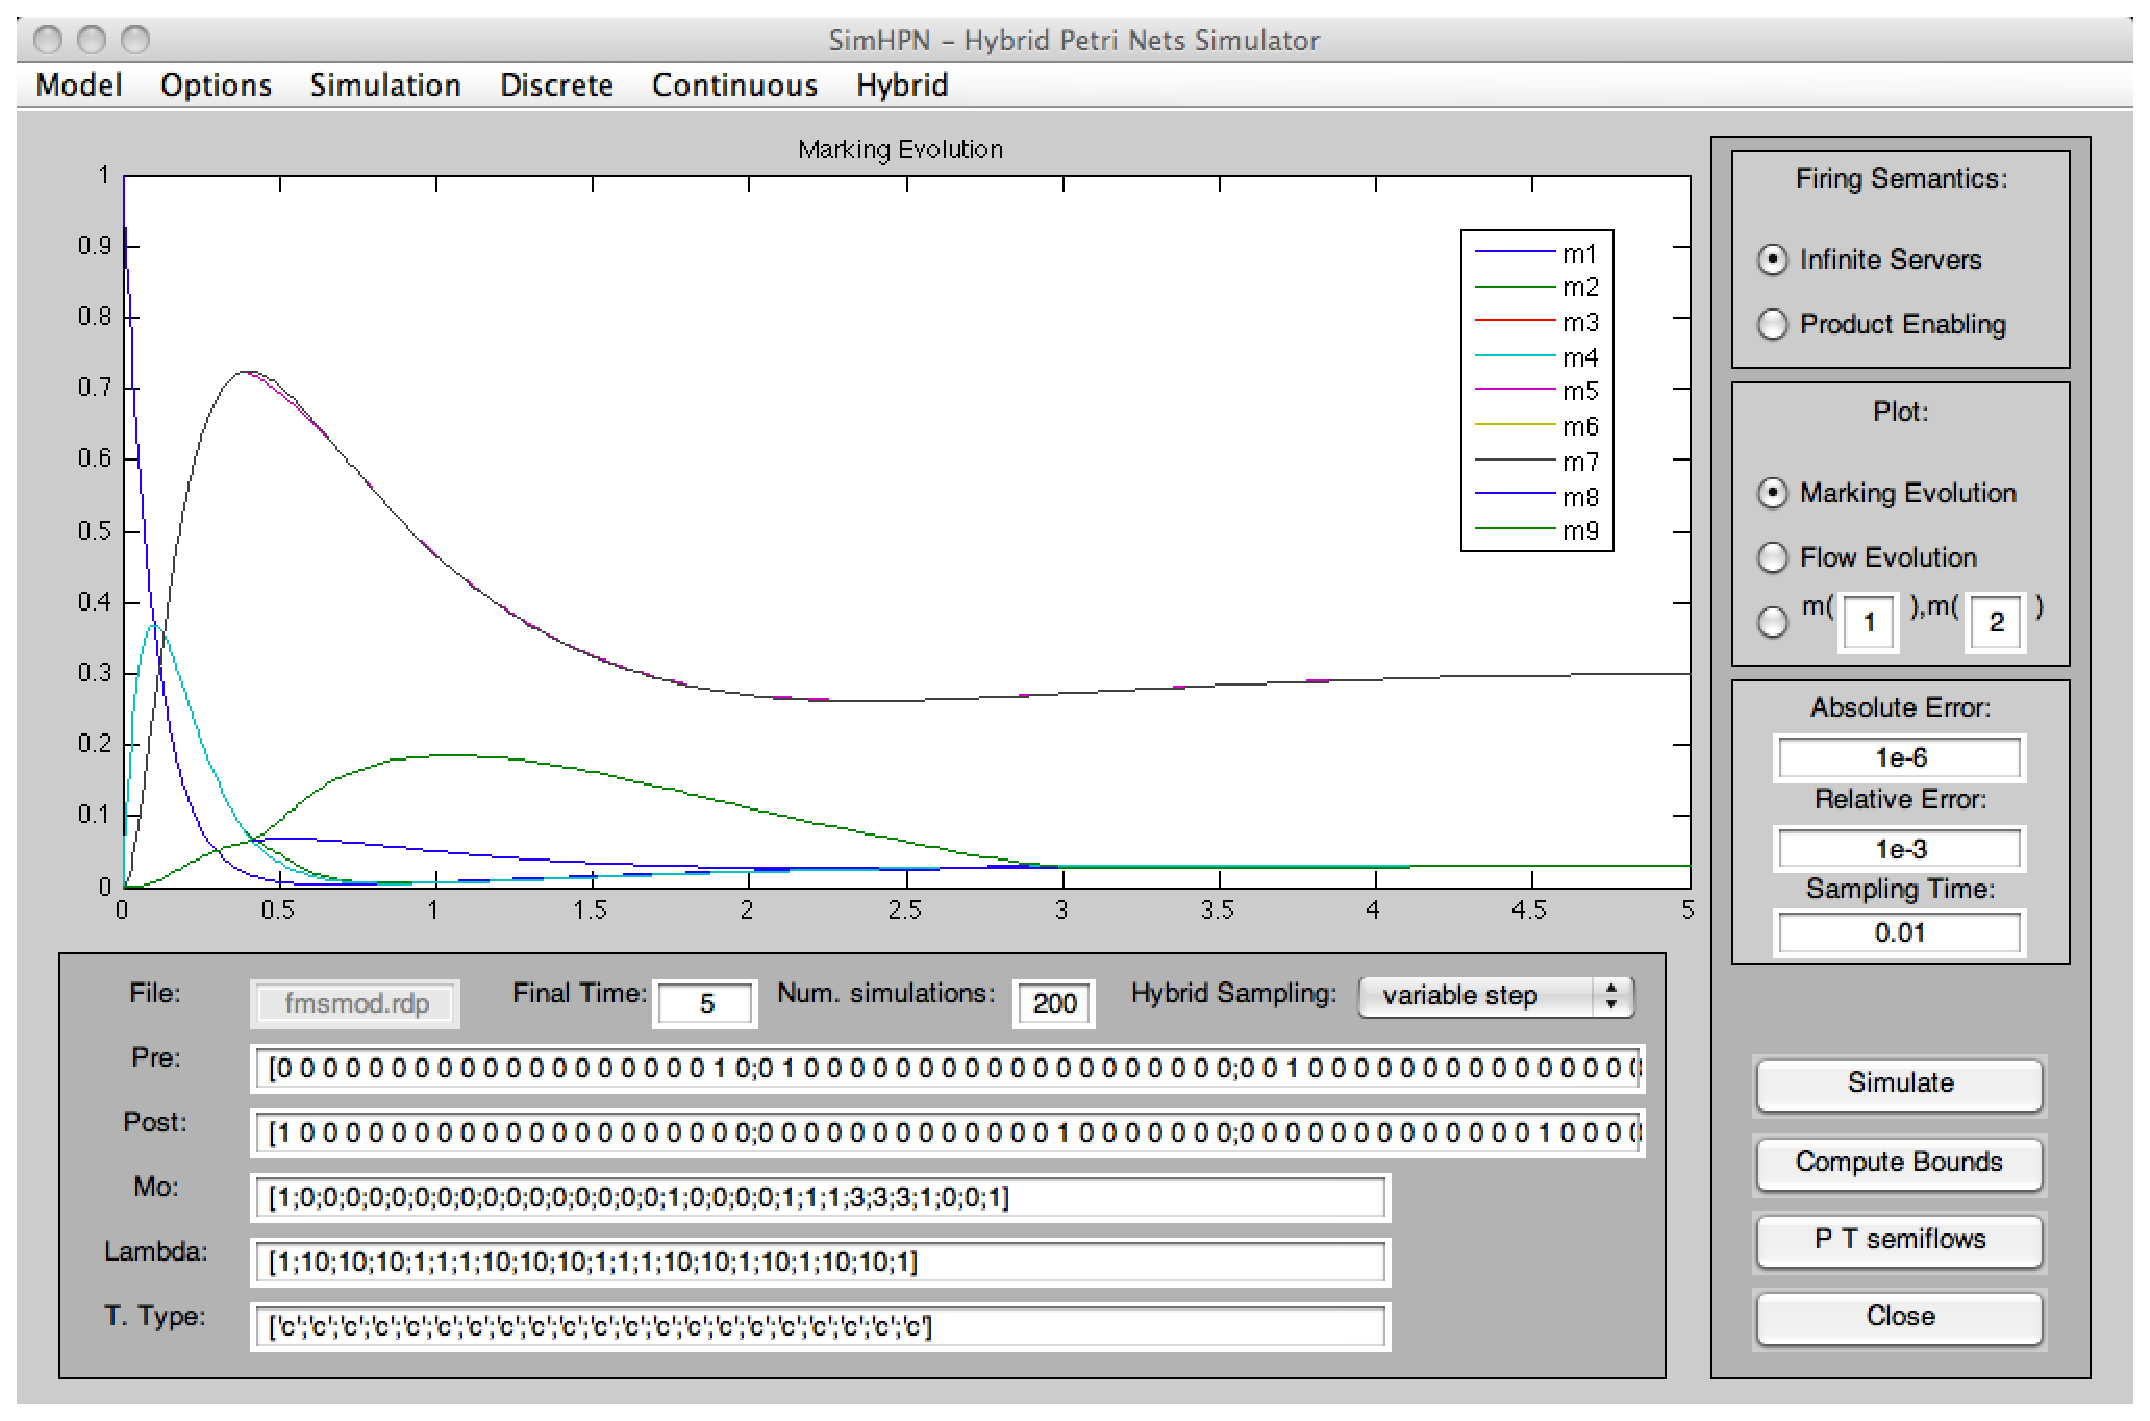
\includegraphics[width=1\columnwidth]{figs/mainScreen.eps}}
   \caption{Sketch of the main window of SimHPN}
   \label{f-main}
\end{figure}


\newpage
